\clearpage
\section{Results}
\label{sec:results}

% TODO introduce results & reiterate RQ

\subsection{Runtime Observations}
\label{subsec:runtime_observations}

\subsection{15-Minute City Metric}
\label{subsec:15_minute_city_metric}

% table (mean, quantiles) of the optimal X-minute city metric
Table \ref{tab:optimal_x_minute_city_metric} shows the mean, as well as, the 25\%, 50\% and 75\% quantiles of the optimal X-minute city disregarding the cost for each scenario.

\begin{table}
  \caption{Optimal X-minute city metric over all hexagons disregarding cost}
  \label{tab:optimal_x_minute_city_metric}
  \begin{center}
    \begin{tabular}{lrrrr}
       & mean & 25\% & 50\% & 75\% \\
      scenario &  &  &  &  \\
      bicycle & 12.45 & 7.25 & 10.75 & 15.50 \\
      bicycle_public_transport & 11.51 & 7.25 & 10.33 & 14.31 \\
      car & 3.21 & 2.00 & 3.00 & 4.00 \\
      public_transport & 12.78 & 9.00 & 12.00 & 16.00 \\
      walking & 14.09 & 9.00 & 12.00 & 17.00 \\
    \end{tabular}
  \end{center}
\end{table}


% TODO not only intersting observations are relevant
We can make a few interesting observations from this table:
First, adding public transport to walking improves the average optimal time it takes to reach all categories by 1 minute and 28 seconds.
From the quantiles we can see that this improvement is not evenly distributed, but only applies to the 25\% worst hexagons.
Specifically we see no improvement from walking to public transport in the 25\% and 50\% quantiles, but a 2-minute improvement in the 75\% quantile.

Similarly, adding public transport to bicycle sharing improves the average optimal time it takes to reach all categories by 43 seconds.
Again, this improvement is not evenly distributed, but only applies to the 25\% worst hexagons.
Specifically we see no improvement from bicycle sharing to public transport in the 25\% and 50\% quantiles, but a 1-minute improvement in the 75\% quantile.
While there is an improvement in the mean and 75\% quantile, it is not as large as the improvement from walking to public transport.

% visualization of the distribution of the optimal X-minute city metric
We can observe a similar pattern when visualizing the distribution of the optimal X-minute city metric in Figure \ref{fig:optimal_x_minute_city_metric}.

\begin{figure}
  \begin{center}
    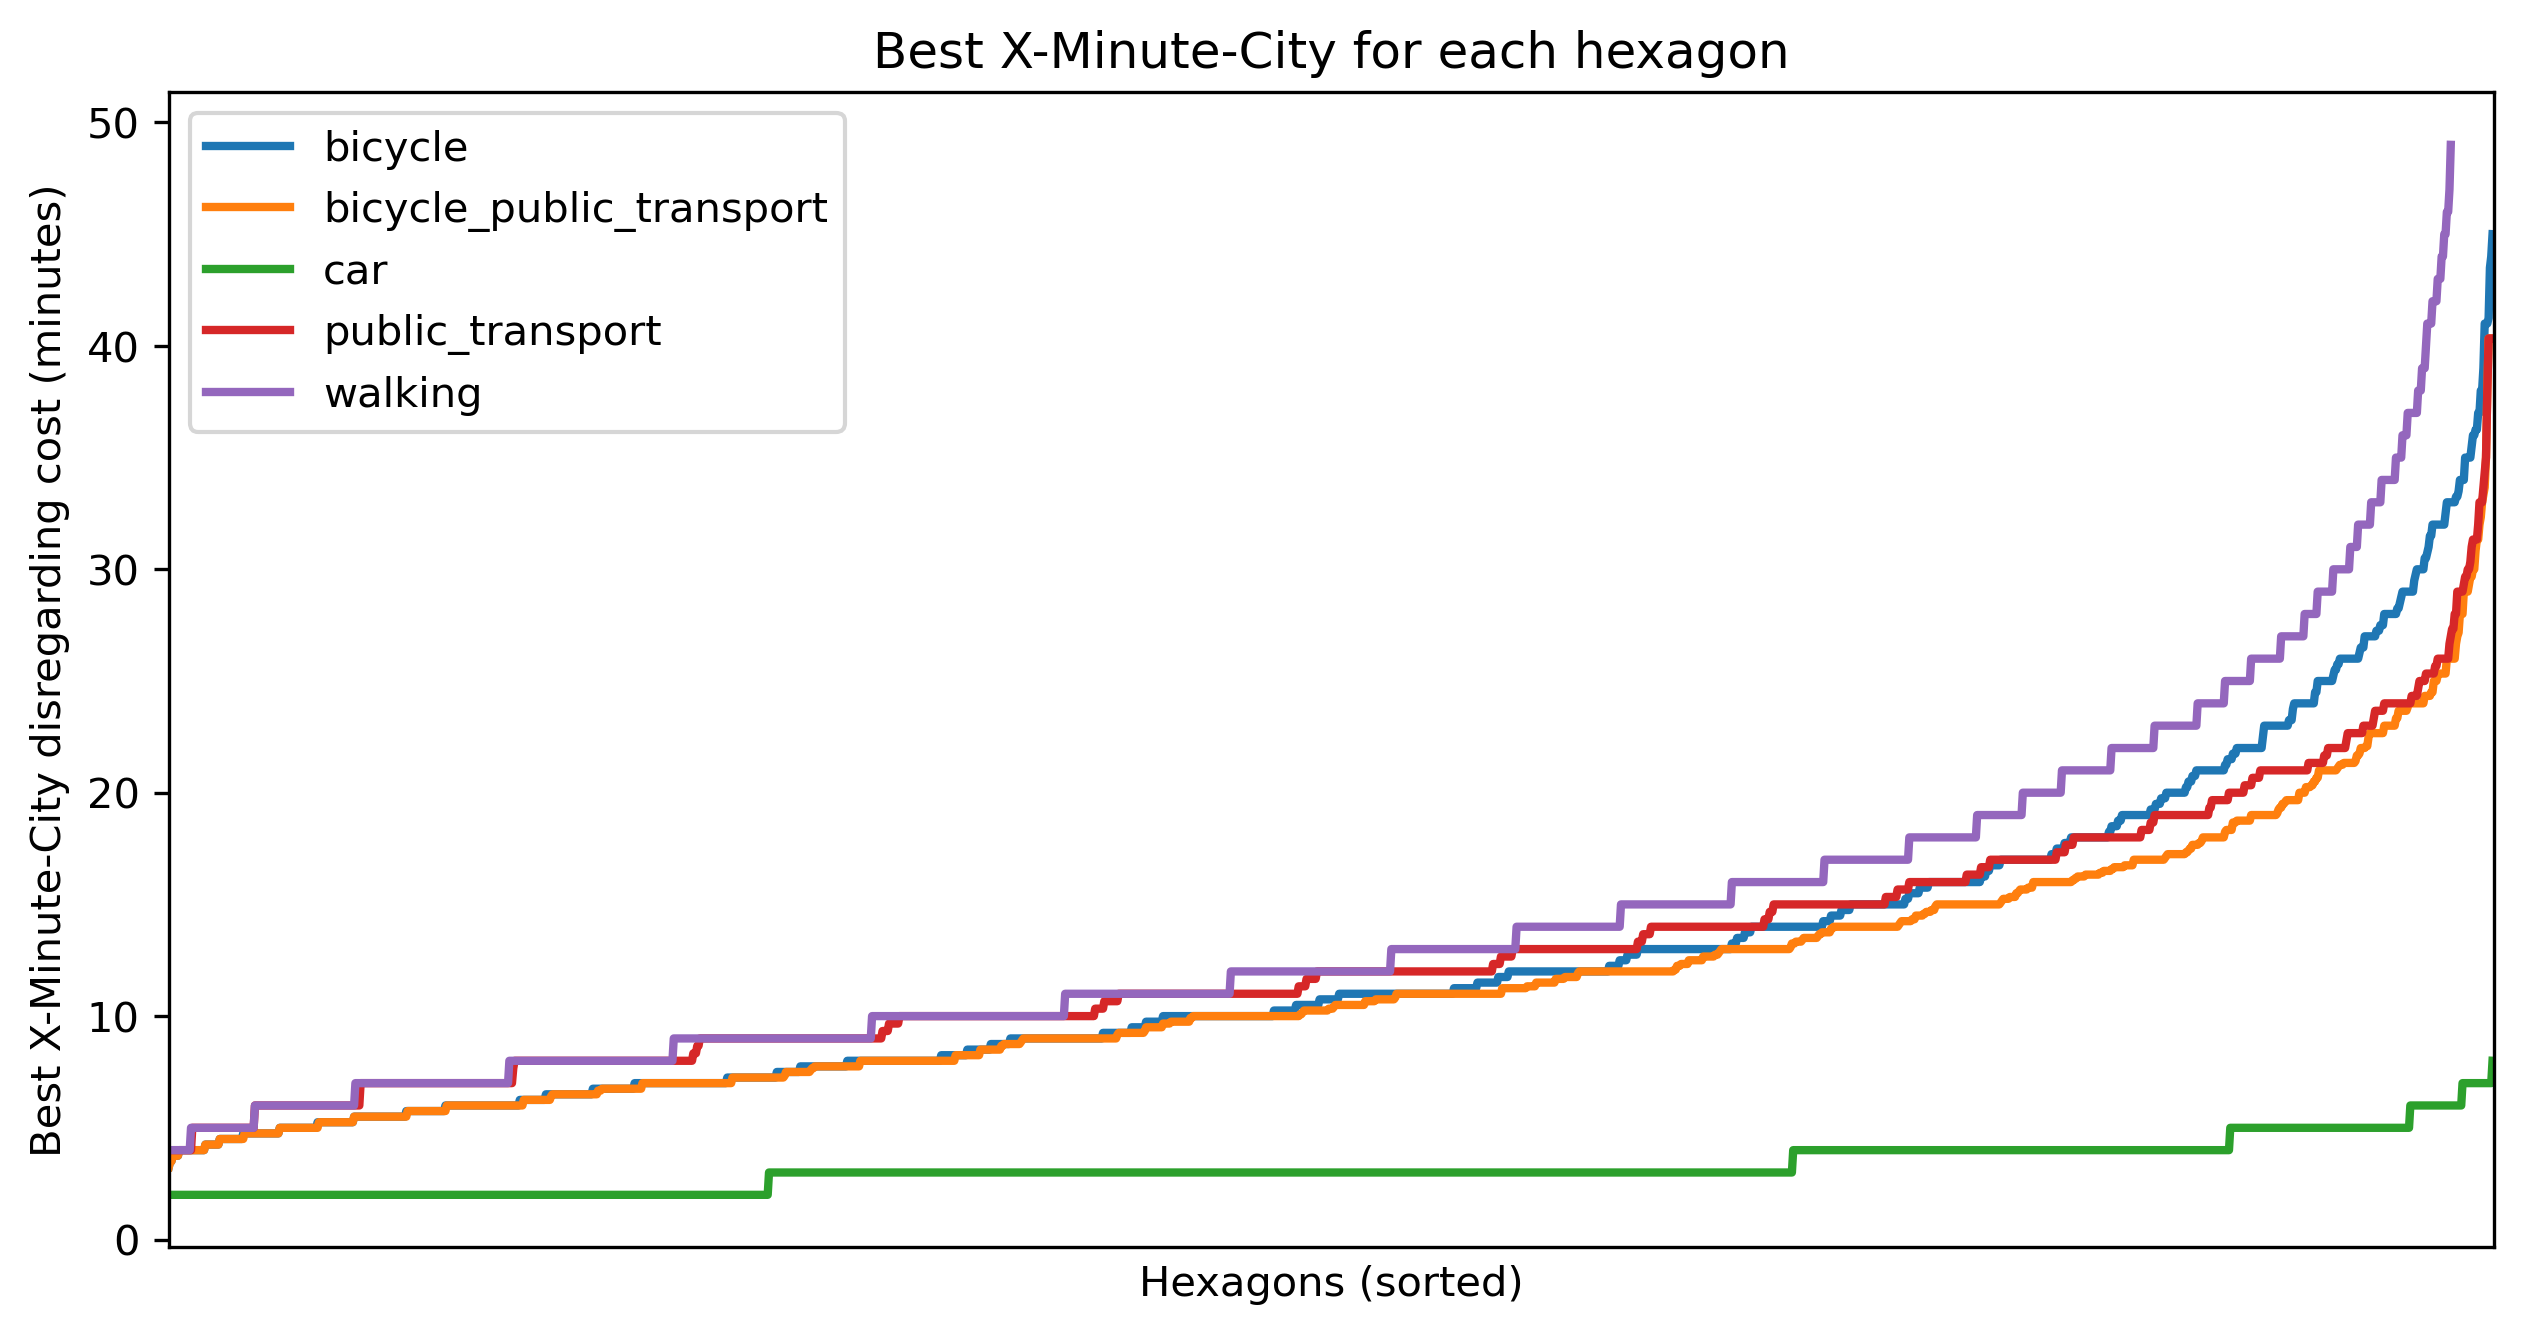
\includegraphics[width=0.65\textwidth]{Figures/results/minute_city_metric/best_x_minute_city}
  \end{center}
  \caption{Distribution of optimal x-minute city metric}
  \label{fig:optimal_x_minute_city_metric}
\end{figure}

As we can see initially (for the most accessible hexagons) public transport and walking are the same, but as we move to less accessible hexagons public transport becomes better.
In addition, the public transport scenario is worse than the pure bicycle sharing scenario, but is able to catch up to it and even overtake it as we move to less accessible hexagons.

The same pattern can be observed when comparing the bicycle sharing scenario to the combined scenario of bicycle sharing and public transport.
Initially, the combined scenario is the same as the bicycle sharing scenario, but as we move to less accessible hexagons the combined scenario becomes better.

Generally, we see that adding public transport is able to flatten the drastic increase of the optimal X-minute city metric at the end of the distribution.


Figure \ref{fig:optimal_map} shows the optimal X-minute city metric for each hexagon over all sustainable modes of travel, i.e. excluding the car scenario.

\begin{figure}
  \begin{center}
    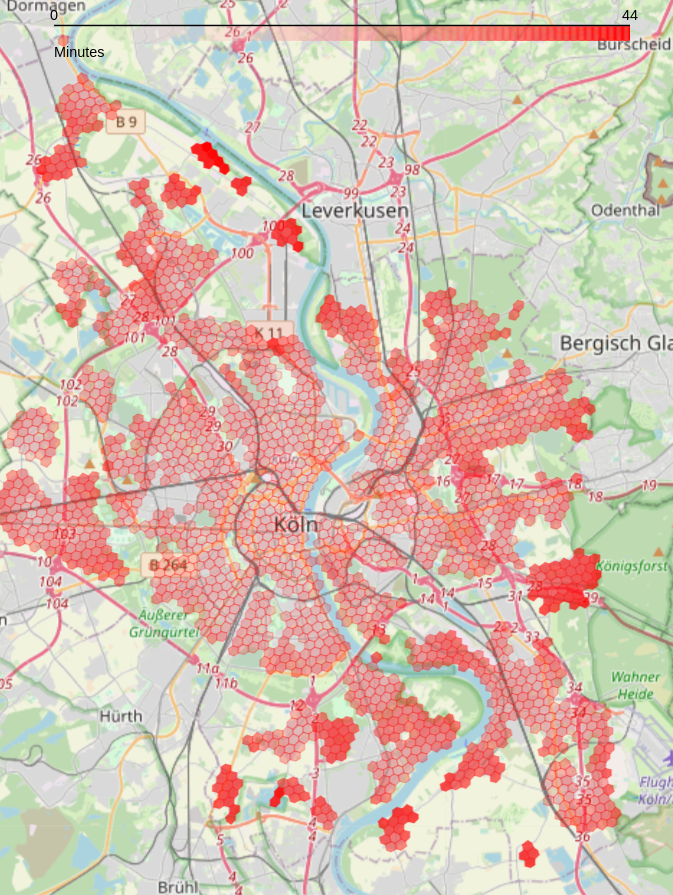
\includegraphics[width=0.45\textwidth]{Figures/results/minute_city_metric/optimal_map}
  \end{center}
  \caption{Map Of Optimal X-Minute City Metric}
  \label{fig:optimal_map}
\end{figure}

We can see that the least accessible hexagons require 44 minutes to reach all categories if only sustainable modes of travel are used.
The least accessible regions are in the suburban areas in the north and south of Cologne. 
Especially the region on the left side of the Rhine river next to Leverkusen is very inaccessible.
% some interpreation (move this to discussion?)
As there are various POIs in the center of Leverkusen and the least accessible regions is very close to the center, this clearly indicates a lack of mobility crossing the Rhine river.
% end of interpretation

Figure \ref{fig:optimal_map_per_scenario} shows multiple maps of the optimal X-minute city metric for each hexagon, one for bicycle sharing, one for public transport and one for walking.

\begin{figure}
     \centering
     \begin{subfigure}[b]{0.3\textwidth}
         \centering
         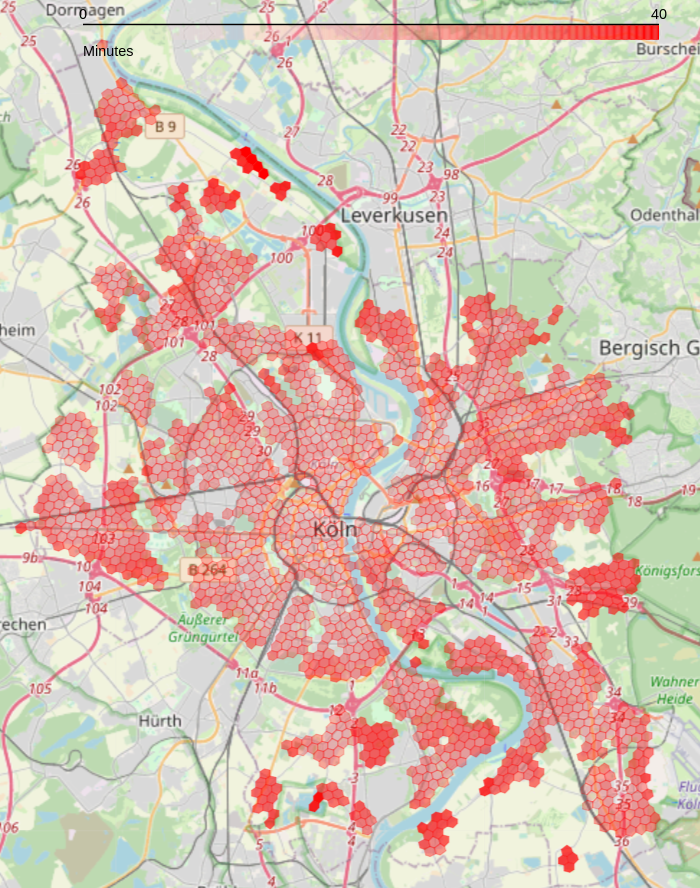
\includegraphics[width=\textwidth]{Figures/results/minute_city_metric/public_transport_optimal_map}
         \caption{Public Transport}
         \label{fig:public_transport_optimal_map}
     \end{subfigure}
     \hfill
     \begin{subfigure}[b]{0.3\textwidth}
         \centering
         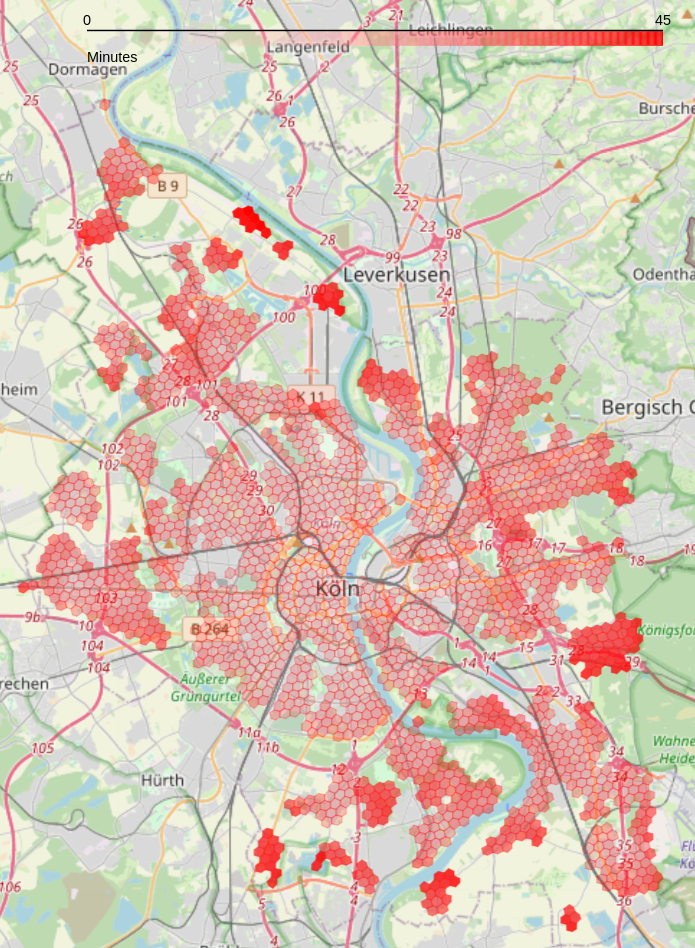
\includegraphics[width=\textwidth]{Figures/results/minute_city_metric/bicycle_optimal_map}
         \caption{Bicycle Sharing}
         \label{fig:bicycle_optimal_map}
     \end{subfigure}
     \hfill
     \begin{subfigure}[b]{0.3\textwidth}
         \centering
         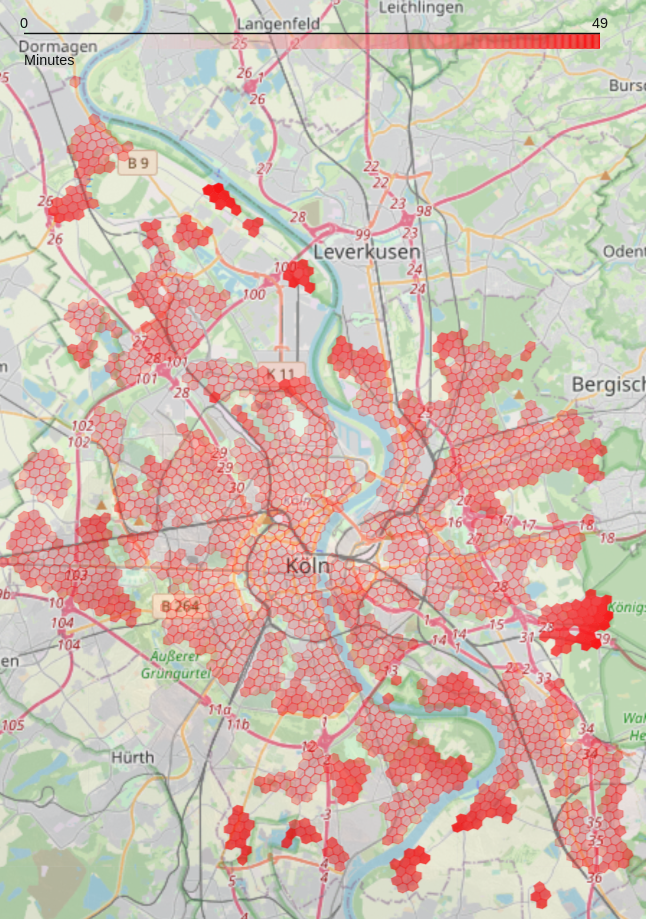
\includegraphics[width=\textwidth]{Figures/results/minute_city_metric/walking_optimal_map}
         \caption{Walking}
         \label{fig:walking_optimal_map}
     \end{subfigure}
        \caption{Map Of Optimal X-Minute City Metric Per Scenario}
        \label{fig:optimal_map_per_scenario}
\end{figure}

We see that the areas in and around the city center are more accessible by bicycle sharing than by public transport and walking.
% some interpreation (move this to discussion?)
This is not surprising, as this area is covered by the NextBike flex zone, i.e. people can park their bicycles anywhere in this area.
This leads to a high availability of bicycles in this area, which in turn leads to a high accessibility.
Also as picking up bicyles requires no waiting time, in comparison to public transport, and is faster than walking, this leads to faster access to POIs.
% end of interpretation

At the east of the city, near the forest "Königsforst", we see a region of low accessibility for all scenarios.
However, one can see that the region is more accessible by public transport than by bicycle sharing and walking.
% some interpreation (move this to discussion?)
This is not surprising, as this region is quite far away from POIs, which makes walking very slow. 
Also, the region is not in NextBike's flex zone, which leads to a low availability of bicycles.
However, the city train line 9 runs through this region, which leads to a higher accessibility by public transport.
% end of interpretation




\subsection{Cost Of 15-Minute City}
\label{subsec:cost_of_15_minute_city}

% table (mean, quantiles) of required cost
Table \ref{tab:required_cost} shows the mean, the 25\%, 50\% and 75\% quantiles and the max of the cost that are required to achieve the optimal value for the X-minute city.

\begin{table}
  \caption{Required cost for optimal over all hexagons}
  \label{tab:required_cost}
  \begin{center}
    \begin{tabular}{lrrrrr}
     & mean & 25\% & 50\% & 75\% & max \\
    scenario &  &  &  &  &  \\
    bicycle & 0.39 & 0.00 & 0.50 & 0.75 & 1.00 \\
    bicycle_public_transport & 0.87 & 0.00 & 0.75 & 1.30 & 3.95 \\
    car & 0.37 & 0.19 & 0.38 & 0.38 & 1.33 \\
    public_transport & 0.65 & 0.00 & 0.00 & 1.47 & 3.20 \\
    walking & 0.00 & 0.00 & 0.00 & 0.00 & 0.00 \\
    \end{tabular}
  \end{center}
\end{table}

We can immediately see that there is no cost for hexagons at the 25\% and 50\% quantile when using public transport.
This means that for those hexagons, no public transport is actually used, as it will not yield any improvements compared to walking.
Looking at the 75\% quantile and the maximum of the required cost for an optimal x-minute city metric for public transport, we see that the benefits we observed earlier come at a cost.

Similarly, comparing bicycle sharing to the combined scenario of bicycle sharing and public transport, we see that the maximum required cost is 4.20€ for the combined scenario, compared to 1.00€ for the bicycle sharing scenario.
This again shows that the benefits of adding public transport come at a cost.

We can make the same observation with more granularity when looking at the distribution of the required cost in Figure \ref{fig:maximum_required_cost_for_x_minute_city}.

\begin{figure}
  \begin{center}
    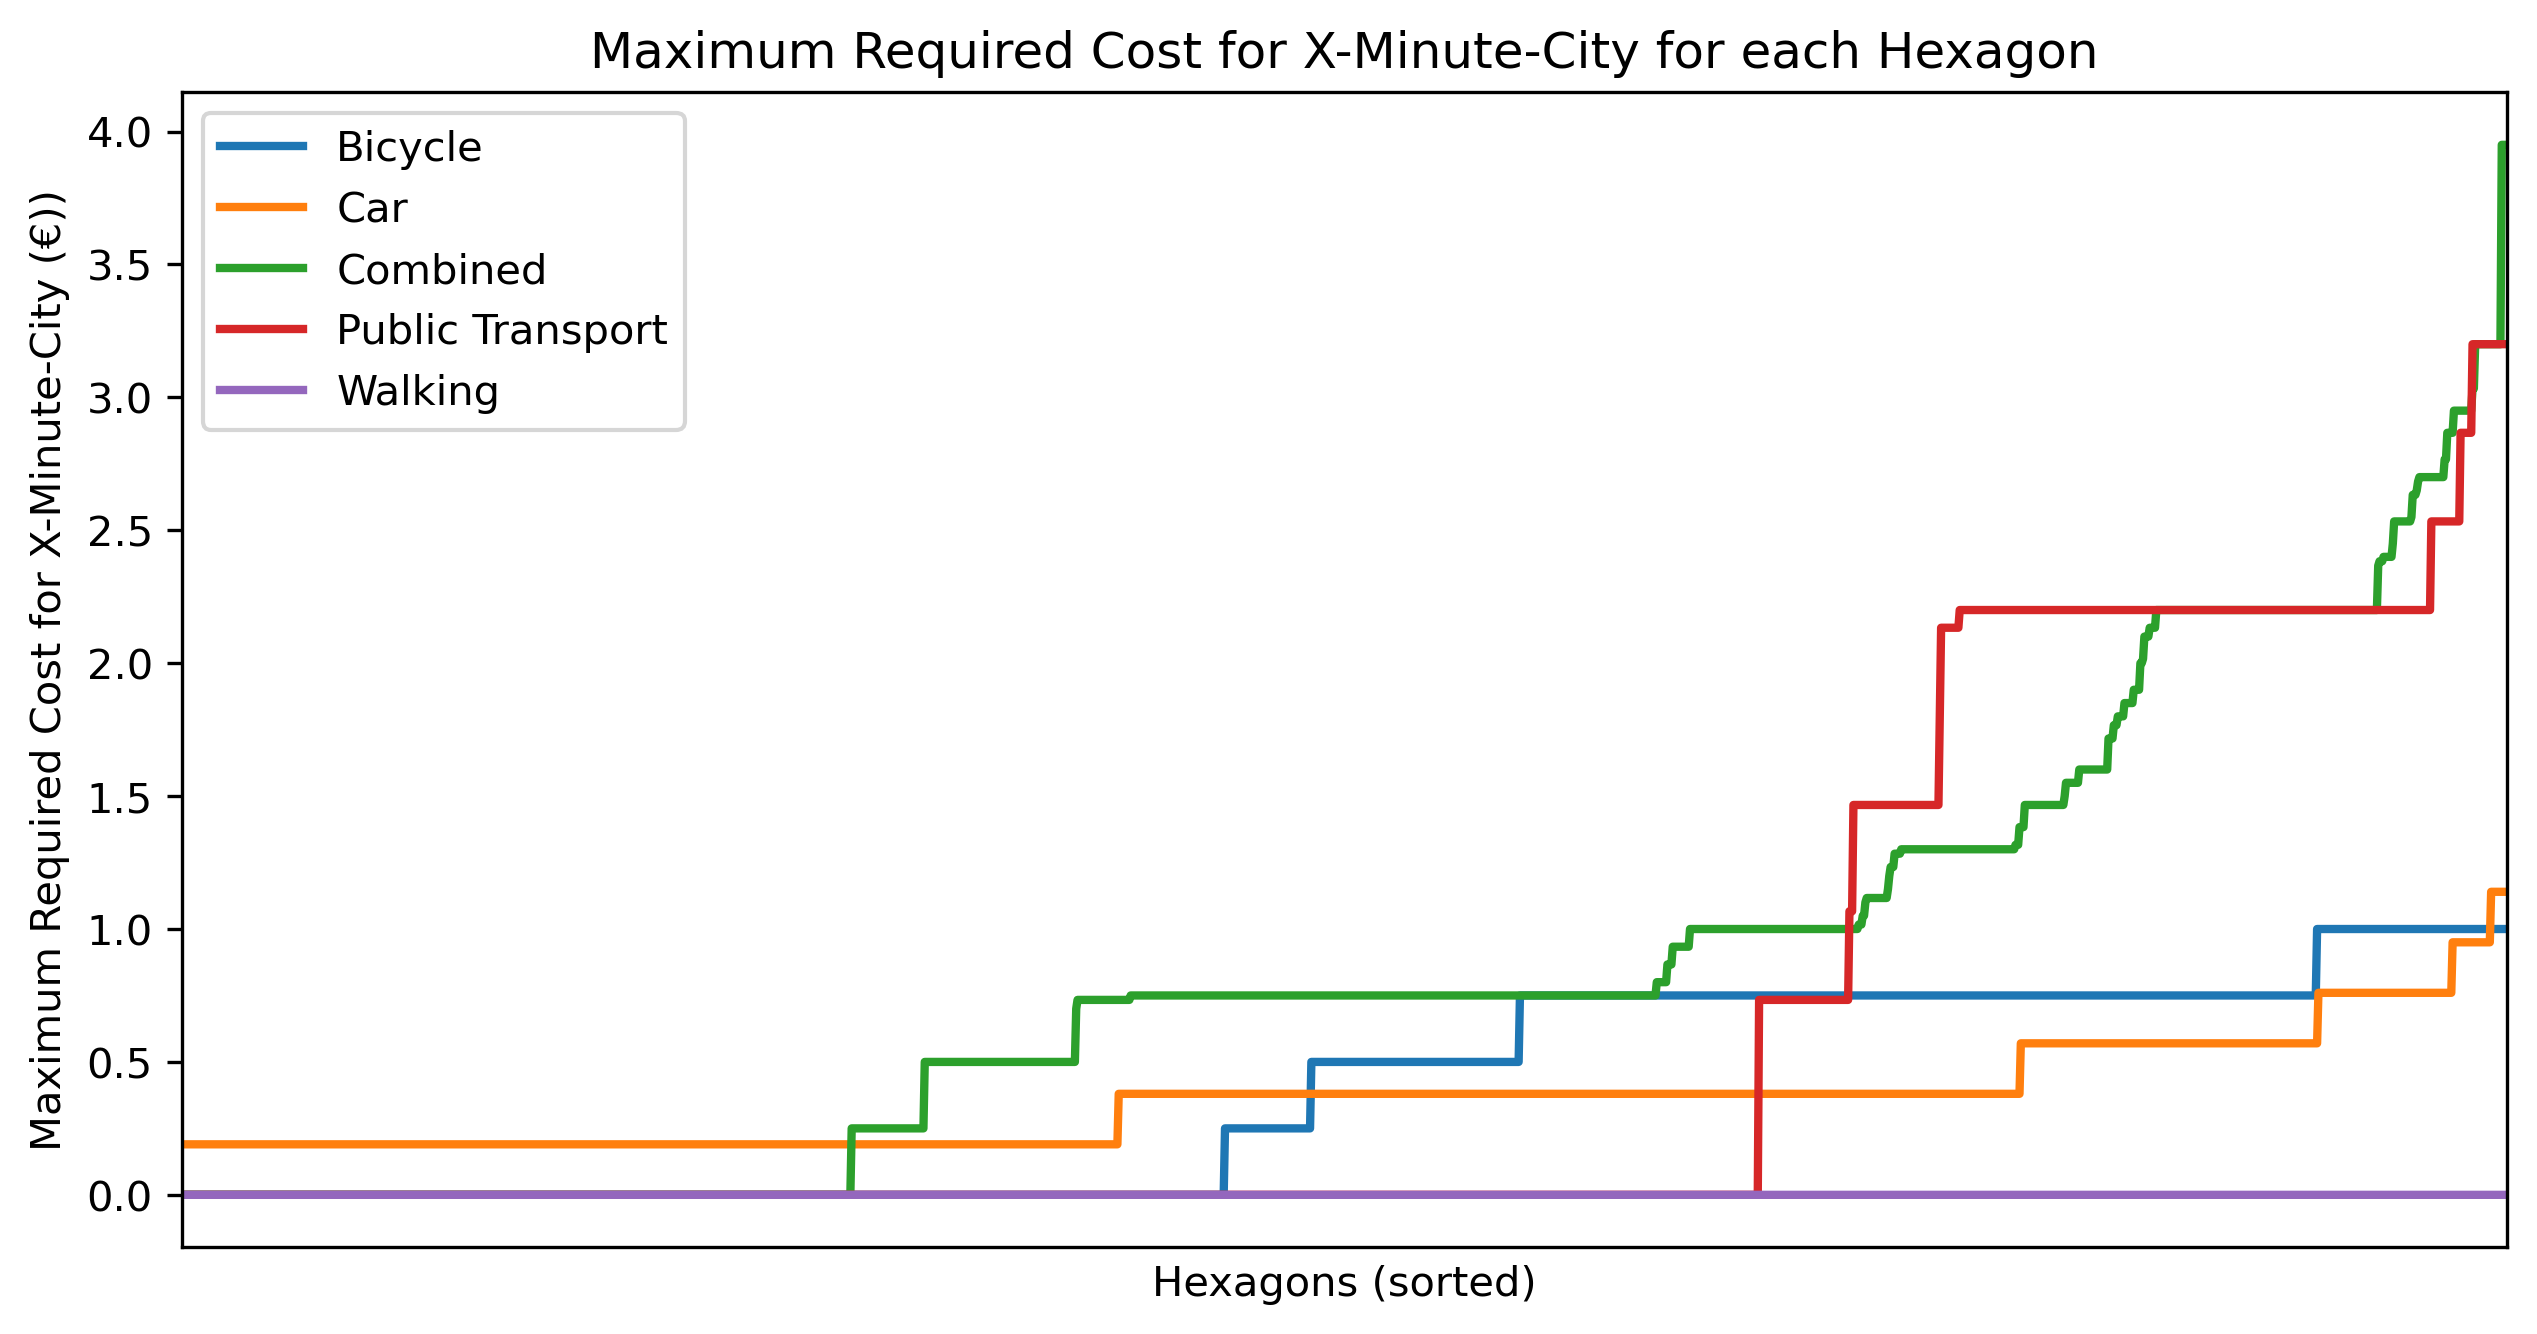
\includegraphics[width=0.65\textwidth]{Figures/results/cost/maximum_required_cost_for_x_minute_city}
  \end{center}
  \caption{Maximum required cost for optimal x-minute city metric}
  \label{fig:maximum_required_cost_for_x_minute_city}
\end{figure}

One interesting remark is that the maximum required cost for the bicycle sharing scenario is 1.00€, which implies that it is never necessary to use a bicycle more than 15 minutes to reach all categories.
This shows that the City of Cologne is already a 15-minute city in terms of cycling at the locations where bicycle sharing is available.


Figure \ref{fig:cost_map_per_scenario} shows the cost required to reach the optimal X-minute city metric for each hexagon for public transport, bicycle sharing and the combined scenario of bicycle sharing and public transport.
Note that, we don't show the cost for the walking scenario, as it is always 0€.

\begin{figure}
     \centering
     \begin{subfigure}[b]{0.3\textwidth}
         \centering
         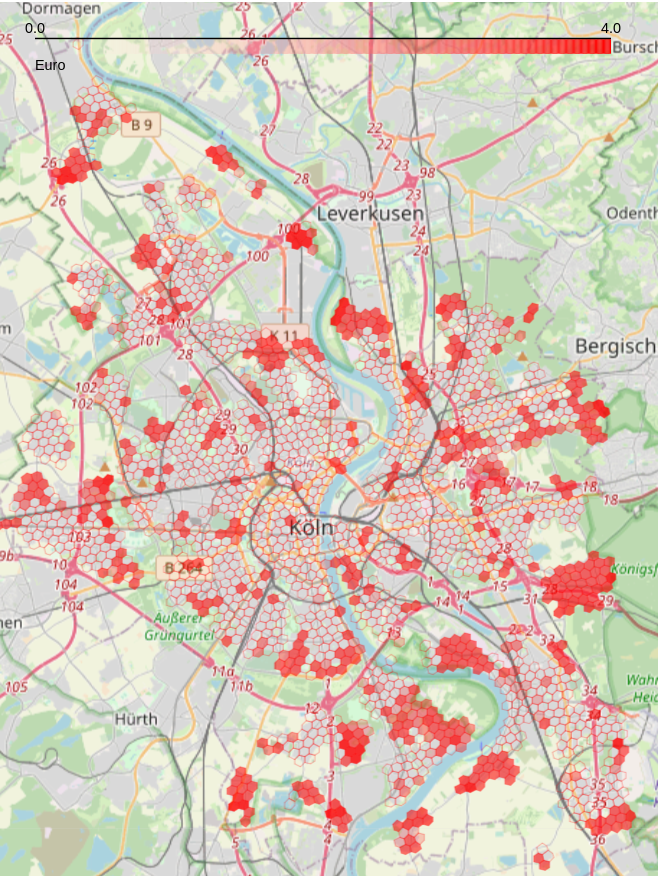
\includegraphics[width=\textwidth]{Figures/results/cost/public_transport_cost_map}
         \caption{Public Transport}
         \label{fig:public_transport_cost_map}
     \end{subfigure}
     \hfill
     \begin{subfigure}[b]{0.3\textwidth}
         \centering
         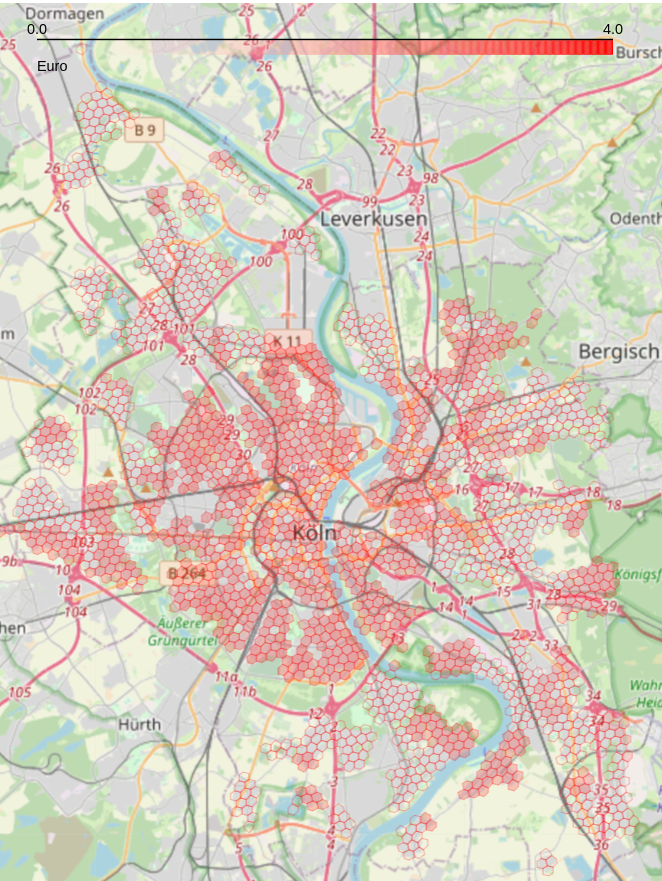
\includegraphics[width=\textwidth]{Figures/results/cost/bicycle_cost_map}
         \caption{Bicycle Sharing}
         \label{fig:bicycle_cost_map}
     \end{subfigure}
     \hfill
     \begin{subfigure}[b]{0.3\textwidth}
         \centering
         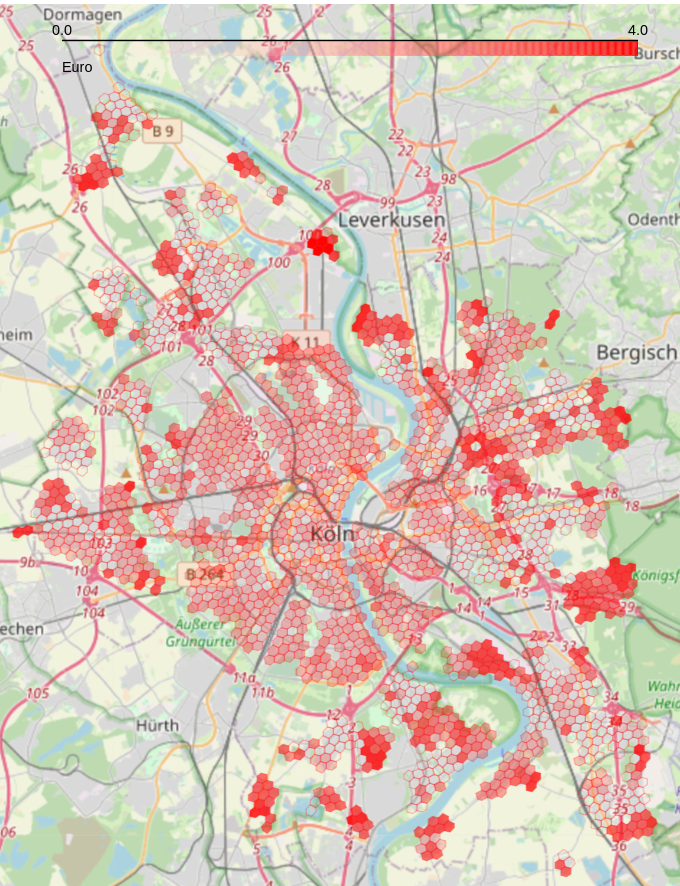
\includegraphics[width=\textwidth]{Figures/results/cost/bicycle_public_transport_cost_map}
         \caption{Walking}
         \label{fig:bicycle_public_transport_cost_map}
     \end{subfigure}
        \caption{Map Of Optimal X-Minute City Metric Per Scenario}
        \label{fig:cost_map_per_scenario}
\end{figure}

In these figures, we see that sometimes the cost is zero.
As the portrayed scenarios all have costs associated with them, a cost of zero means that only walking is used.

We see almost in all hexagons in and around the city center, where NextBike's flex zone is located, the cost for the bicycle sharing scenario is 1.00€.
This sometimes also extends outside the city center.
Other hexagons have a cost of 0.
% some interpreation (move this to discussion?)
The time advantage of bicycle sharing over public transport comes with a cost and we can see exactly that this is the case in the areas, where bicycle sharing is available.
% end of interpretation

The cost of public transport is more scattered around the whole region. We can mostly see single hexagons or small groups of hexagons that have a cost higher than 0.
Larger groups are only found outside the city center.
% some interpreation (move this to discussion?)
The single hexagons are most likely located very close to a public transport stop, enabling to use the public transport system without any loss of time.
Inside the city it seems to only be beneficial to use the public tranport system to reach necessesities when living near a stop.
However, outside the city the larger groups of hexagons indicate that using the public transport system is often faster than walking to the necessities, eventhough walking to the next stop requires some time.
This may be, because the density of the POIs is lower outside the city.
% end of interpretation


\subsection{Interaction Between Cost And 15-Minute City Metric}
\label{subsec:interaction_between_cost_and_15_minute_city_metric}

Next we are going to look at the interaction between the cost and the optimal X-minute city metric.
To do so we will investigate the mean Pareto front of the X-minute city metric and cost over all hexagons.
To understand this graph, we first take a look at the Pareto Front of a single hexagon.

Figure \ref{fig:example_pareto_front} shows an example Pareto Front for a single hexagon.
The x-axes show the cost and the y-axes show the X-minute city metric.
The curves show us what X-minute city is achievable for a given cost in specific scenario.

\begin{figure}
  \begin{center}
     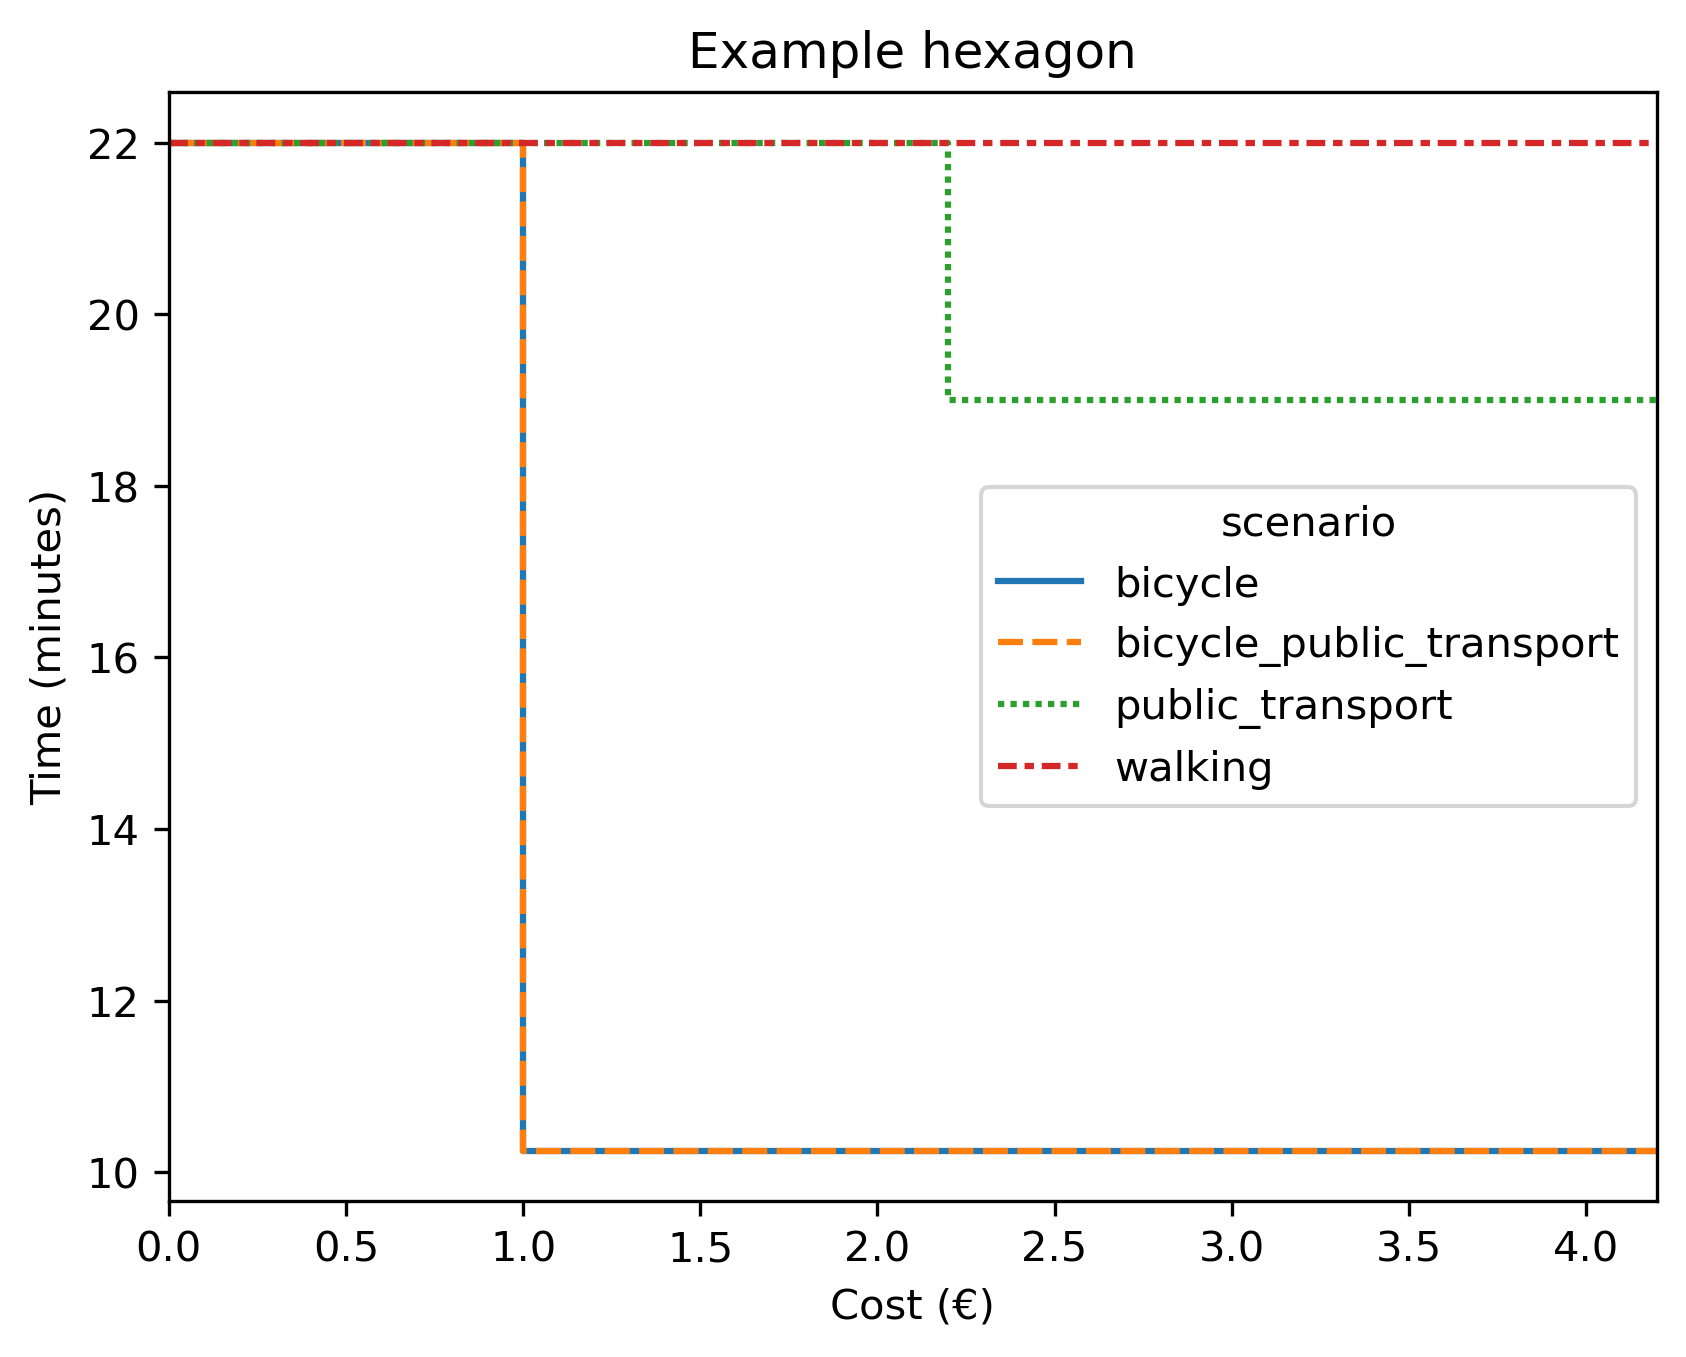
\includegraphics[width=0.5\textwidth]{Figures/results/metric_cost/example_profile}
  \end{center}
  \caption{Example Pareto Front}
  \label{fig:example_pareto_front}
\end{figure}

In our example, all modes begin with being able to reach all categories within 22 minutes for a cost of 0€.
Increasing, the cost only yields improves when reaching a cost of 1€, where the bicycle and combined scenario are able to reach all categories within approximately 10 minutes.
Further, increasing the price to 2.20€ yields an improvement for the public transport scenario, where it is now possible to reach all categories within approximately 19 minutes.
Further cost increases do not yield any improvements for any scenario.
% some interpreation (move this to discussion?)
In this example, we can clearly see that when users are able to afford a bicycle for 15 minutes (cost of 1€), their accessibility to POIs increases drastically.
Similarly, when users are able to afford a short public transport trip (cost of 2.20€), their accessibility to POIs also increases.
% end of interpretation

We can also quantify the value of the improvements as seen in Table \ref{tab:differences_in_example_hexagon}.

\begin{table}
  \caption{Differences in example hexagon}
  \label{tab:differences_in_example_hexagon}
  \begin{center}
    \begin{tabular}{lrrrl}
    improvement & at cost & minute per euro & scenario \\
    11.75 & 1.00 & 11.75 & bicycle \\
    11.75 & 1.00 & 11.75 & bicycle_public_transport \\
    3.00 & 2.20 & 1.36 & public_transport \\
    \end{tabular}
  \end{center}
\end{table}

As we can see the bicycle scenarios' increase at a cost of 1€ is larger than the public transport scenario's increase and also has a higher value per euro.


% generalization
To generalize these findings over all hexagons we take the average over the X-minute city for each cost and scenario to generate an average Pareto front.
The resulting Pareto front can be seen in Figure \ref{fig:mean_time_per_cost}.

\begin{figure}
  \begin{center}
     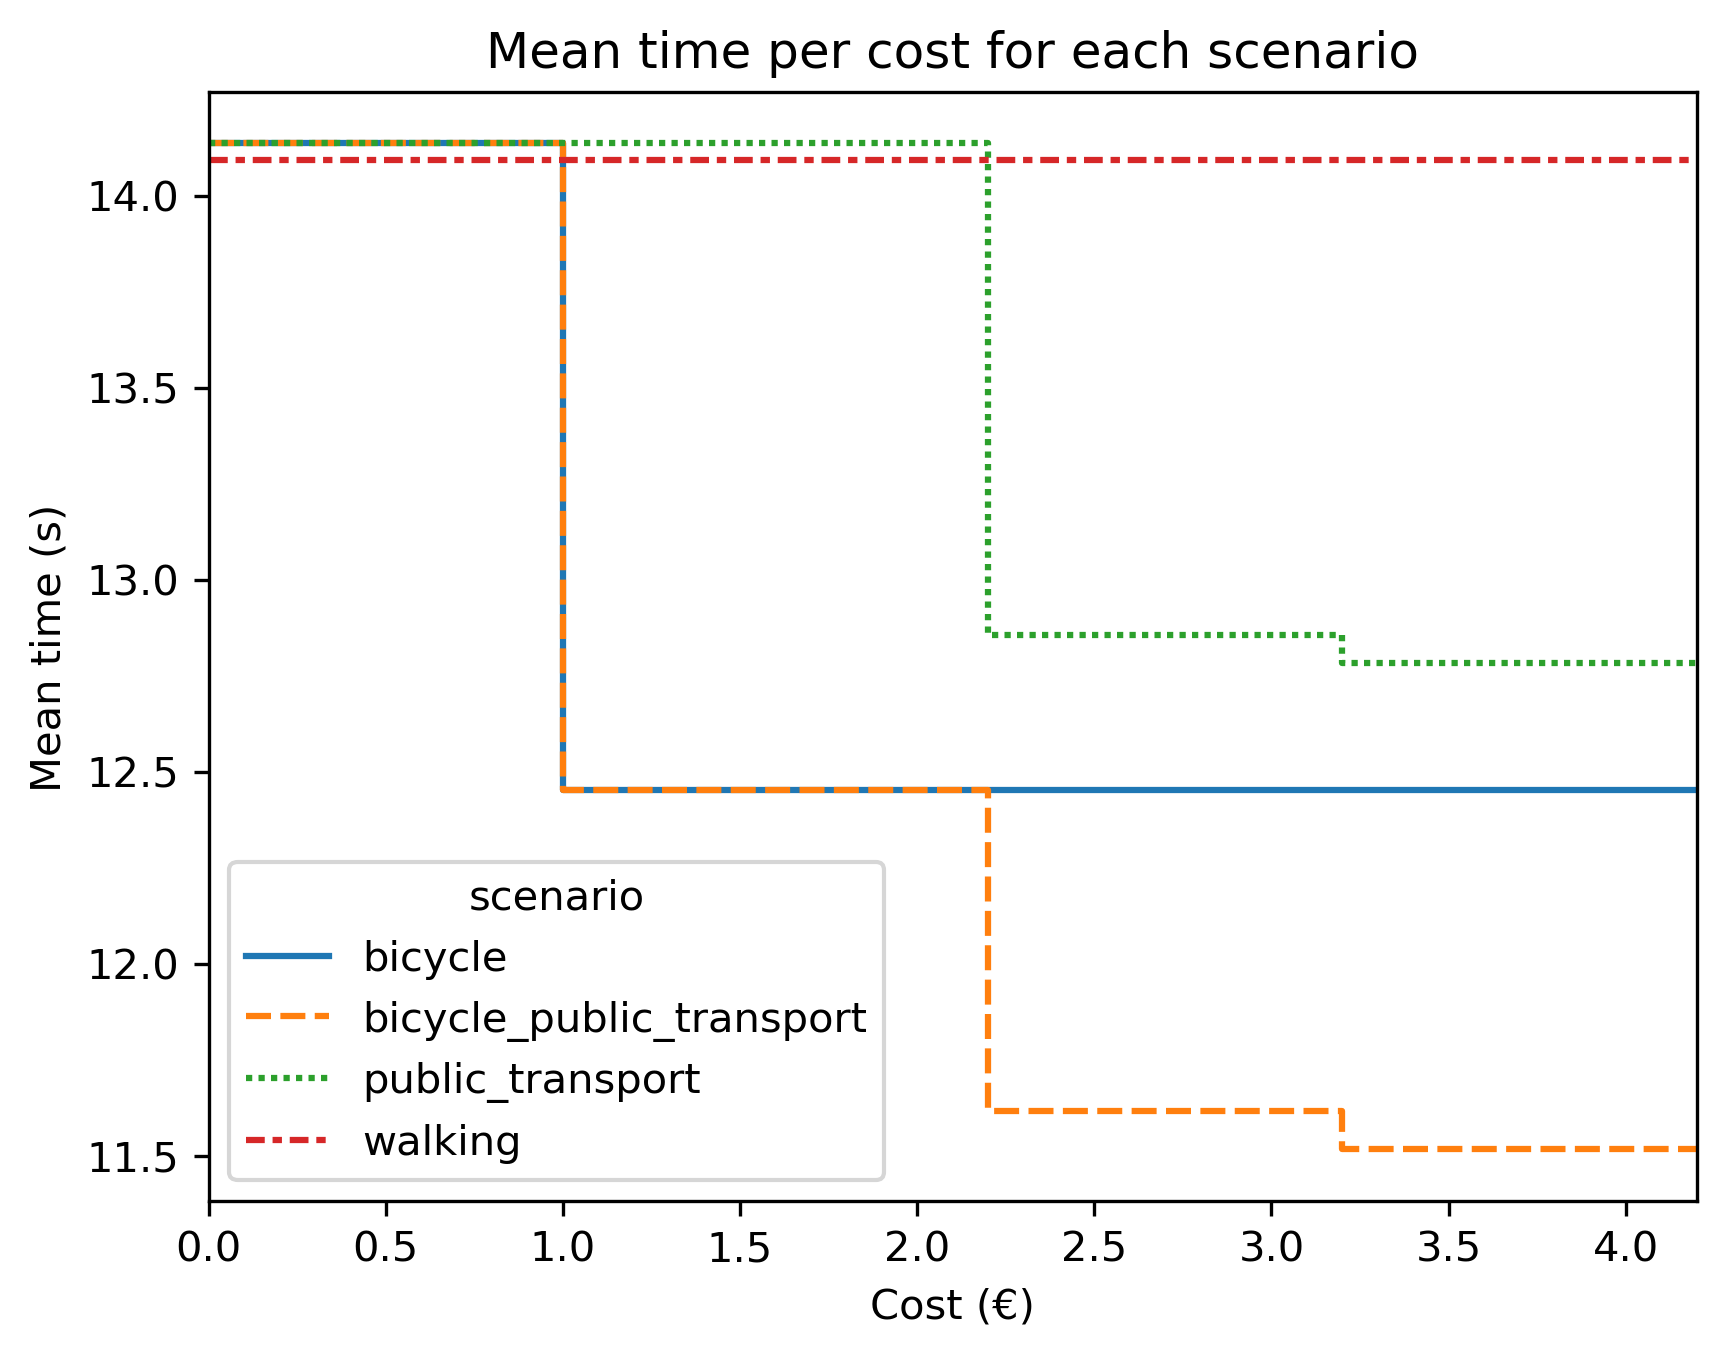
\includegraphics[width=0.5\textwidth]{Figures/results/metric_cost/mean_time_per_cost}
  \end{center}
  \caption{Mean time per cost for all scenarios}
  \label{fig:mean_time_per_cost}
\end{figure}

Similarly to the example of the single hexagon from before, we can see improvements for the bicycle scenario, as well as, the combined scenario at a cost of 1€ of about 1.5 minutes.
We can also see the improvements of public transport at a cost of 2.20€.
Unlike the example of the single hexagon, we can also see the improvement at a cost of 2.20€ for the combined scenario.
Lastly, there is also a slight improvement for the public transport scenario, as well as, the combined scenario at a cost of 3.20€.

To compare these improvements we can again look at the differences in Table \ref{tab:differences_in_mean_pareto_front}.
Note that we won't be analyzing the differences that occur in the combined scenario, as they may be skewed by prior improvements of other modes and are therefore hard to interpret.

\begin{table}
  \caption{Differences in mean Pareto front}
  \label{tab:differences_in_mean_pareto_front}
  \begin{center}
    \begin{tabular}{lrrrrl}
     & improvement & at cost & cost diff & minute per euro & scenario \\
     & 1.684 & 1.000 & 1.000 & 1.684 & bicycle \\
     & 1.282 & 2.200 & 2.200 & 0.583 & public transport \\
     & 0.074 & 3.200 & 1.000 & 0.074 & public transport \\
    \end{tabular}
  \end{center}
\end{table}

We see that the improvements of the bicycle scenarios at a cost of 1€ are the largest with an improvement of 1.68 minutes and also the most cost-effective with a value of 1.68 minutes per euro.
They are followed by the improvements of the public transport scenario at a cost of 2.20€ with an improvement of 1.28 minutes and a value of 0.58 minutes per euro.
The improvement at a cost of 3.20€ is very small and the least cost-effective.


% some interpreation (move this to discussion?)
This observation underlines the importance and price-effectiveness of bicycle sharing.
It also shows us that public transport for most areas is more useful when the trips are short, i.e. four stops or fewer and that longer trips only yield a small improvement on average.
% end of interpretation

Next, we are going to look at the quantiles of the aggregated Pareto front.
Figure \ref{fig:quantile_time_per_cost} shows the 25\%, 75\% and 90\% quantiles of the aggregated Pareto front.
The 25\% quantile gives us insights about the more accessible areas in the city.
Note that, because we aggregate all the values of the X-minute city metric for a single cost and scenario at a time, the 25\% quantile Pareto front does not necessarily reflect the same 25\% of hexagons for each cost.

\begin{figure}
     \centering
     \begin{subfigure}[b]{0.48\textwidth}
         \centering
         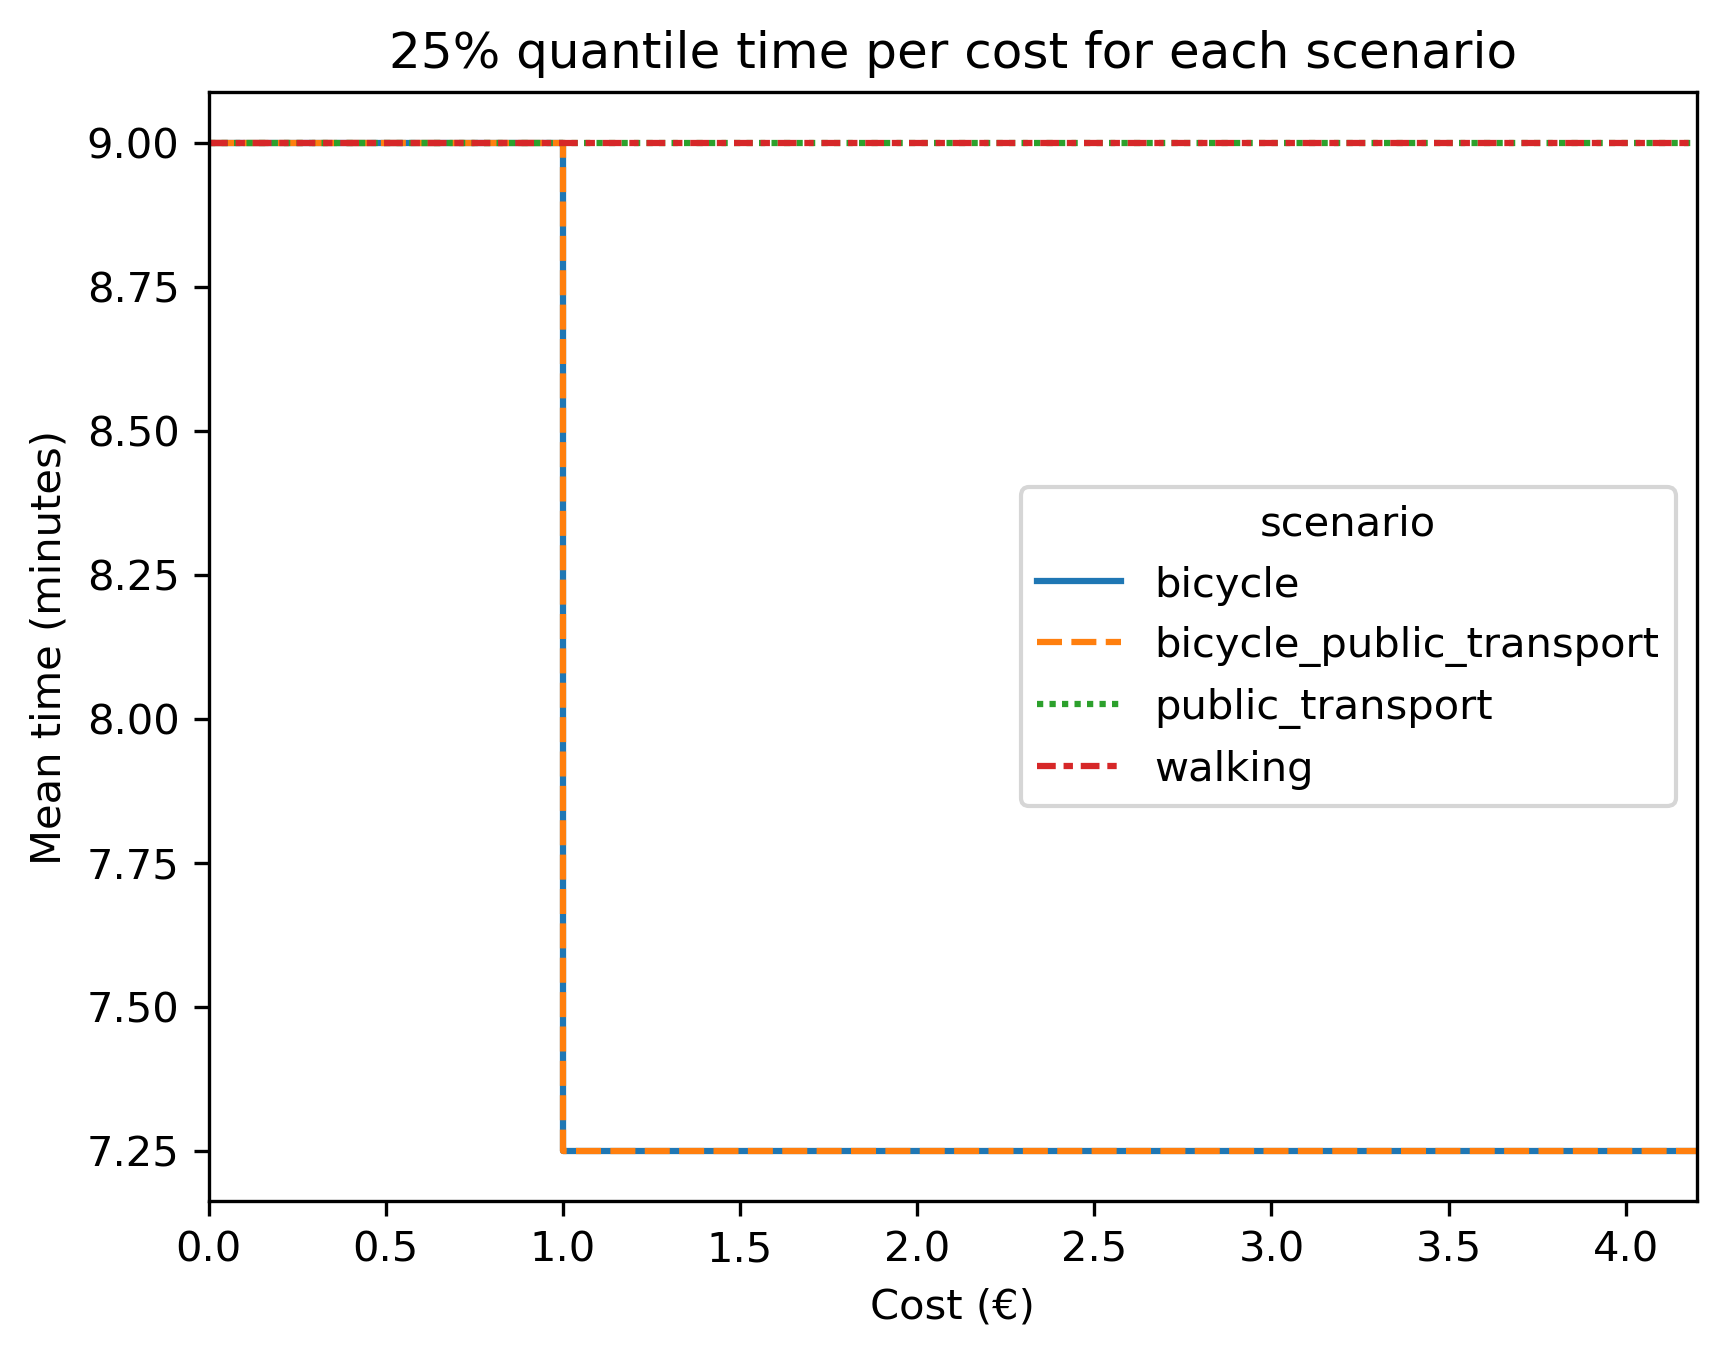
\includegraphics[width=\textwidth]{Figures/results/metric_cost/quantile_25_time_per_cost_for_each_scenario_without_car.png}
         \caption{25\% quantile time per cost for all scenarios}
         \label{fig:25_quantile_time_per_cost}
     \end{subfigure}
     \hfill
     \begin{subfigure}[b]{0.48\textwidth}
         \centering
         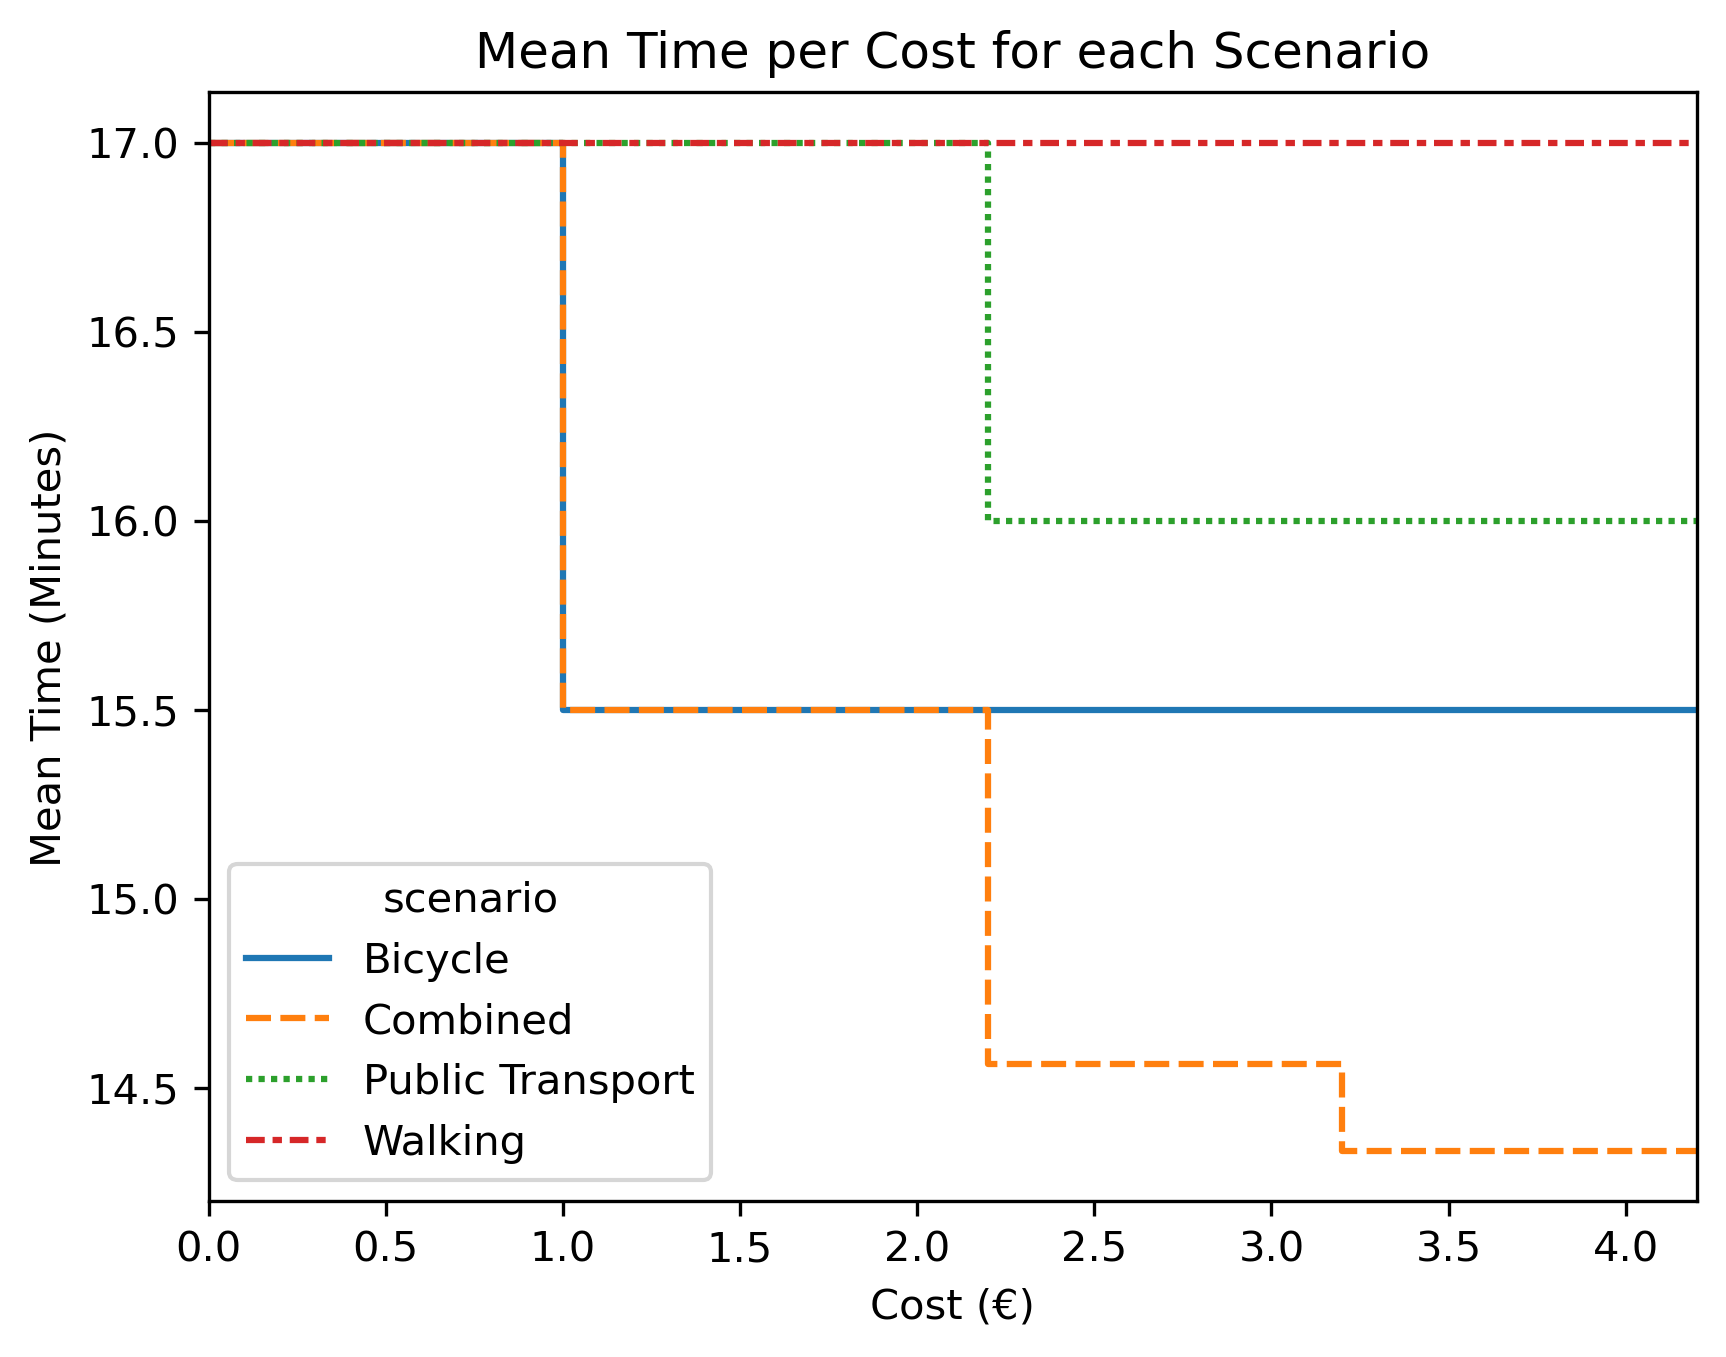
\includegraphics[width=\textwidth]{Figures/results/metric_cost/quantile_75_time_per_cost_for_each_scenario_without_car.png}
         \caption{75\% quantile time per cost for all scenarios}
         \label{fig:75_quantile_time_per_cost}
     \end{subfigure}
     \hfill
     \begin{subfigure}[b]{0.48\textwidth}
         \centering
         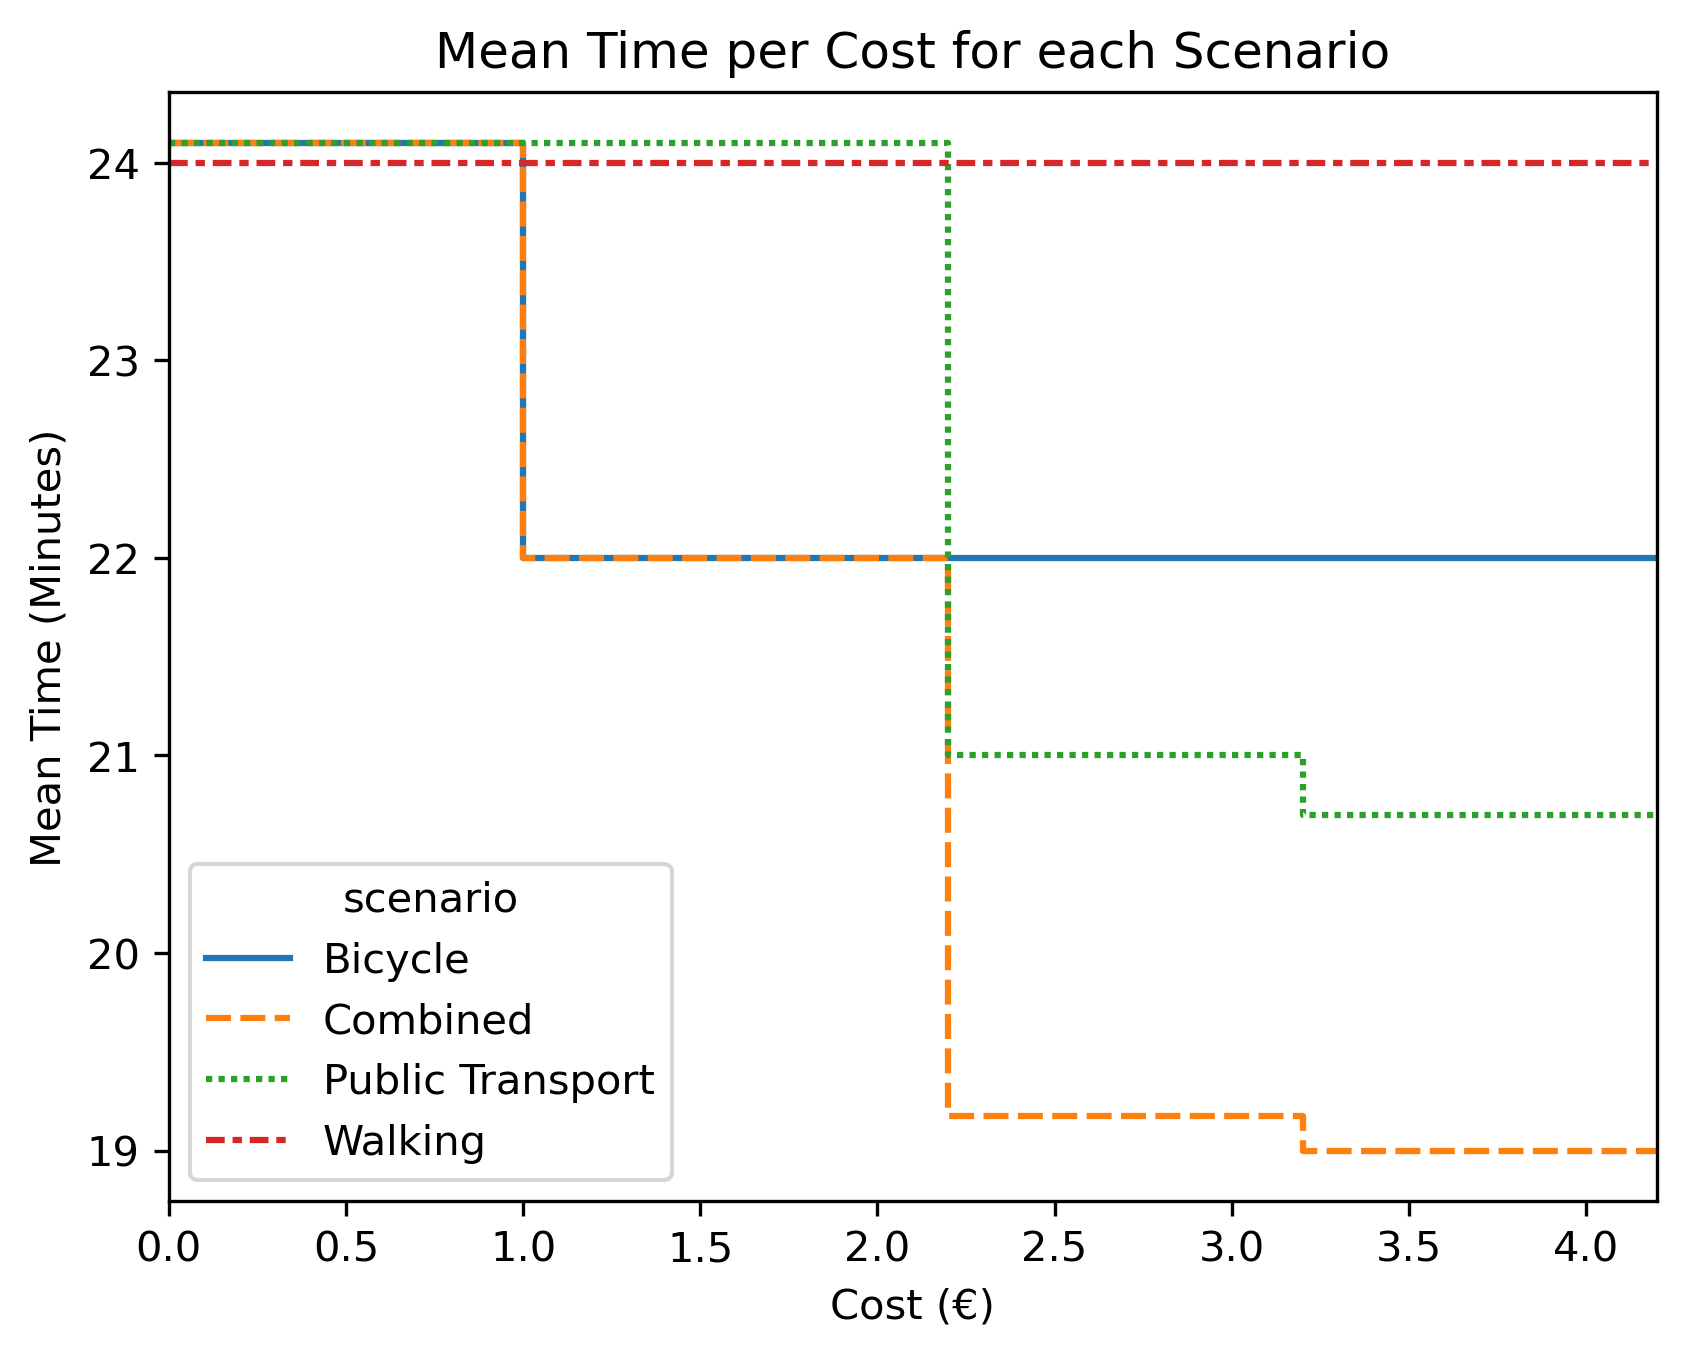
\includegraphics[width=\textwidth]{Figures/results/metric_cost/quantile_90_time_per_cost_for_each_scenario_without_car.png}
         \caption{90\% quantile time per cost for all scenarios}
         \label{fig:90_quantile_time_per_cost}
     \end{subfigure}
        \caption{Map Of Optimal X-Minute City Metric Per Scenario}
        \label{fig:quantile_time_per_cost}
\end{figure}

The 25\% quantile Pareto front shown in Figure \ref{fig:25_quantile_time_per_cost} only contains a single improvement at the cost of 1€ for bicycle related scenarios of 1.75 minutes with a cost-effectiveness of 1.75 minutes per euro.


The 75\% quantile Pareto front shown in Figure \ref{fig:75_quantile_time_per_cost} and Table \ref{tab:differences_in_75_quantile_pareto_front} also has a similar improvement of 1.5 minutes at the cost of 1€ for bicycle scenarios.
In addition to that, it also shows a smaller increase at 2.20€ for public transport scenarios of 1 minute and an even smaller increase at 3.20€ for bicycle sharing and public transport scenario.

\begin{table}
  \caption{Differences in 75\% quantile Pareto front}
  \label{tab:differences_in_75_quantile_pareto_front}
  \begin{center}
    \begin{tabular}{lrrrrl}
     improvement & at cost & cost diff & minute per euro & scenario \\
     1.500 & 1.000 & 1.000 & 1.500 & bicycle \\
     1.000 & 2.200 & 2.200 & 0.455 & public transport \\
    \end{tabular}
  \end{center}
\end{table}


The 90\% quantile Pareto Front shown in Figure \ref{fig:90_quantile_time_per_cost} and Table \ref{tab:differences_in_90_quantile_pareto_front} shows a similar pattern to the 75\% quantile Pareto front.
The major difference is that the increase at 2.20€ for public transport scenarios is larger than the increase at 1€ for bicycle scenarios.
More precisely, while bicycle sharing is more effective in decreasing the 15-minute city metric on average and also for the 75\% most accessible regions, public transport is more effective than bicycle sharing for the 10\% least accessible regions.
We should, however, note that even though the improvement in the public transport scenario is larger it is still less cost-effective than the improvement in the bicycle sharing scenario.


\begin{table}
  \caption{Differences in 90\% quantile Pareto front}
  \label{tab:differences_in_90_quantile_pareto_front}
  \begin{center}
    \begin{tabular}{lrrrrl}
     improvement & at cost & cost diff & minute per euro & scenario \\
     3.000 & 2.200 & 2.200 & 1.364 & public transport \\
     2.000 & 1.000 & 1.000 & 2.000 & bicycle \\
     0.033 & 3.200 & 1.000 & 0.033 & public transport \\
    \end{tabular}
  \end{center}
\end{table}

% some interpreation (move this to discussion?)
In general, bicycle sharing brings larger improvements than public transport, while remaining more cost-effective.
The improvements of bicycle sharing are effective for the most accessible regions, while the improvements of public transport are not.
This shows that extending the bicycle sharing system might be a good way to improve the accessibility in Cologne.

However, for the least accessible regions, public transport is more effective than bicycle sharing.
This most likely means that there are regions in the region of Cologne, where some categories of POIs are not present.
We suspect that those regions are characterized by low accessibility and low or no availability of bicycles.
In those regions public transport becomes more effective than bicycles, as it essentially allows to relocate to better areas.
In the spirit of the 15-minute city, it might be more desirable to fix the sparsity of POIs than to substitute public transport.
% end of interpretation



\subsection{Uncertainty/Subscenarios}
\label{subsec:uncertainty_subscenarios}

As some of our input data is subject to uncertainties, we need to investigate the effects of this uncertainty in order to establish the robustness of our results.

First, we are going to look at the average standard deviation of the optimal value for the X-minute city metric in Table \ref{tab:average_standard_deviation_of_optimal_value_for_x_minute_city_metric}, effectively showing the standard deviation of the values in Table \ref{tab:optimal_x_minute_city_metric}.
Note, that we display the average standard deviations of the bicycle, public transport and combined scenario as those are the only ones with uncertainty.

\begin{table}
  \caption{Average standard deviation of optimal value for X-minute city metric}
  \label{tab:average_standard_deviation_of_optimal_value_for_x_minute_city_metric}
  \begin{center}
    \begin{tabular}{lrrrrrrr}
     & mean & min & 25\% & 50\% & 75\% & max & CV \\
    scenario &  &  &  &  &  &  &  \\
    bicycle & 1.16 & 0.00 & 0.00 & 0.50 & 1.73 & 13.15 & 0.093403 \\
    bicycle_public_transport & 0.94 & 0.00 & 0.00 & 0.74 & 1.48 & 6.73 & 0.082027 \\
    public_transport & 0.27 & 0.00 & 0.00 & 0.00 & 0.00 & 8.66 & 0.021151 \\
    \end{tabular}
  \end{center}
\end{table}


We see that the mean average standard deviation for bicycle scenarios is around a minute, while it is 0.27 for the public transport scenario.
We can also see that for the bicycle related scenarios the uncertainty does not affect the 25\% most accessible hexagons, while for public transport the 75\% most accessible hexagons are not affected.
In addition, we see that outliers exist with more than 10 minutes of deviation for the pure bicycle scenario and more than 5 minutes of deviation for the public transport related scenarios.
Relating the standard deviation to the mean we also calculated the Coefficient of Variation (CV) to the table, which is calculated as follows:
$$ CV = \frac{\sigma}{\mu} $$
where $\mu$ is the mean and $\sigma$ is the standard deviation.
We see that it is approximately 9\% for the bicycle related scenarios and 2\% for the public transport scenario.

% some interpreation (move this to discussion?)
A deviation of one minute on average with a CV of $<10\%$ is acceptable.
It is interesting to note that bicycles suffer more from uncertainty than public transport. 
However, this might strongly depend on the choices of our sub-scenarios. 
For public transport we tried 08:00, 12:00 and 18:00.
We suspect that the variance for public transport would increase more drastically and eventually surpass the one of bicycle sharing if we choose more unusual times like midnight.
We should also note that the comparison of variances should be taken with caution as the method for selecting the sub-scenarios differ per scenario.
For bicycle sharing we employed a clustering method, while for public transport we made a qualitative choice. 
% end of interpretation


To further investigate the effects of uncertainty on a more granular level, we plot the distribution of the optimal X-minute city for each hexagon in Figure \ref{fig:best_and_worst_case_of_optimal_time_for_each_hexagon}.
These plots are essentially the upper and lower bounds of the graph as seen in Figure \ref{fig:optimal_x_minute_city_metric}.
In addition, we've added a line at the 15-minute mark, to better relate the results in context of the 15-minute city.


\begin{figure}
  \begin{center}
    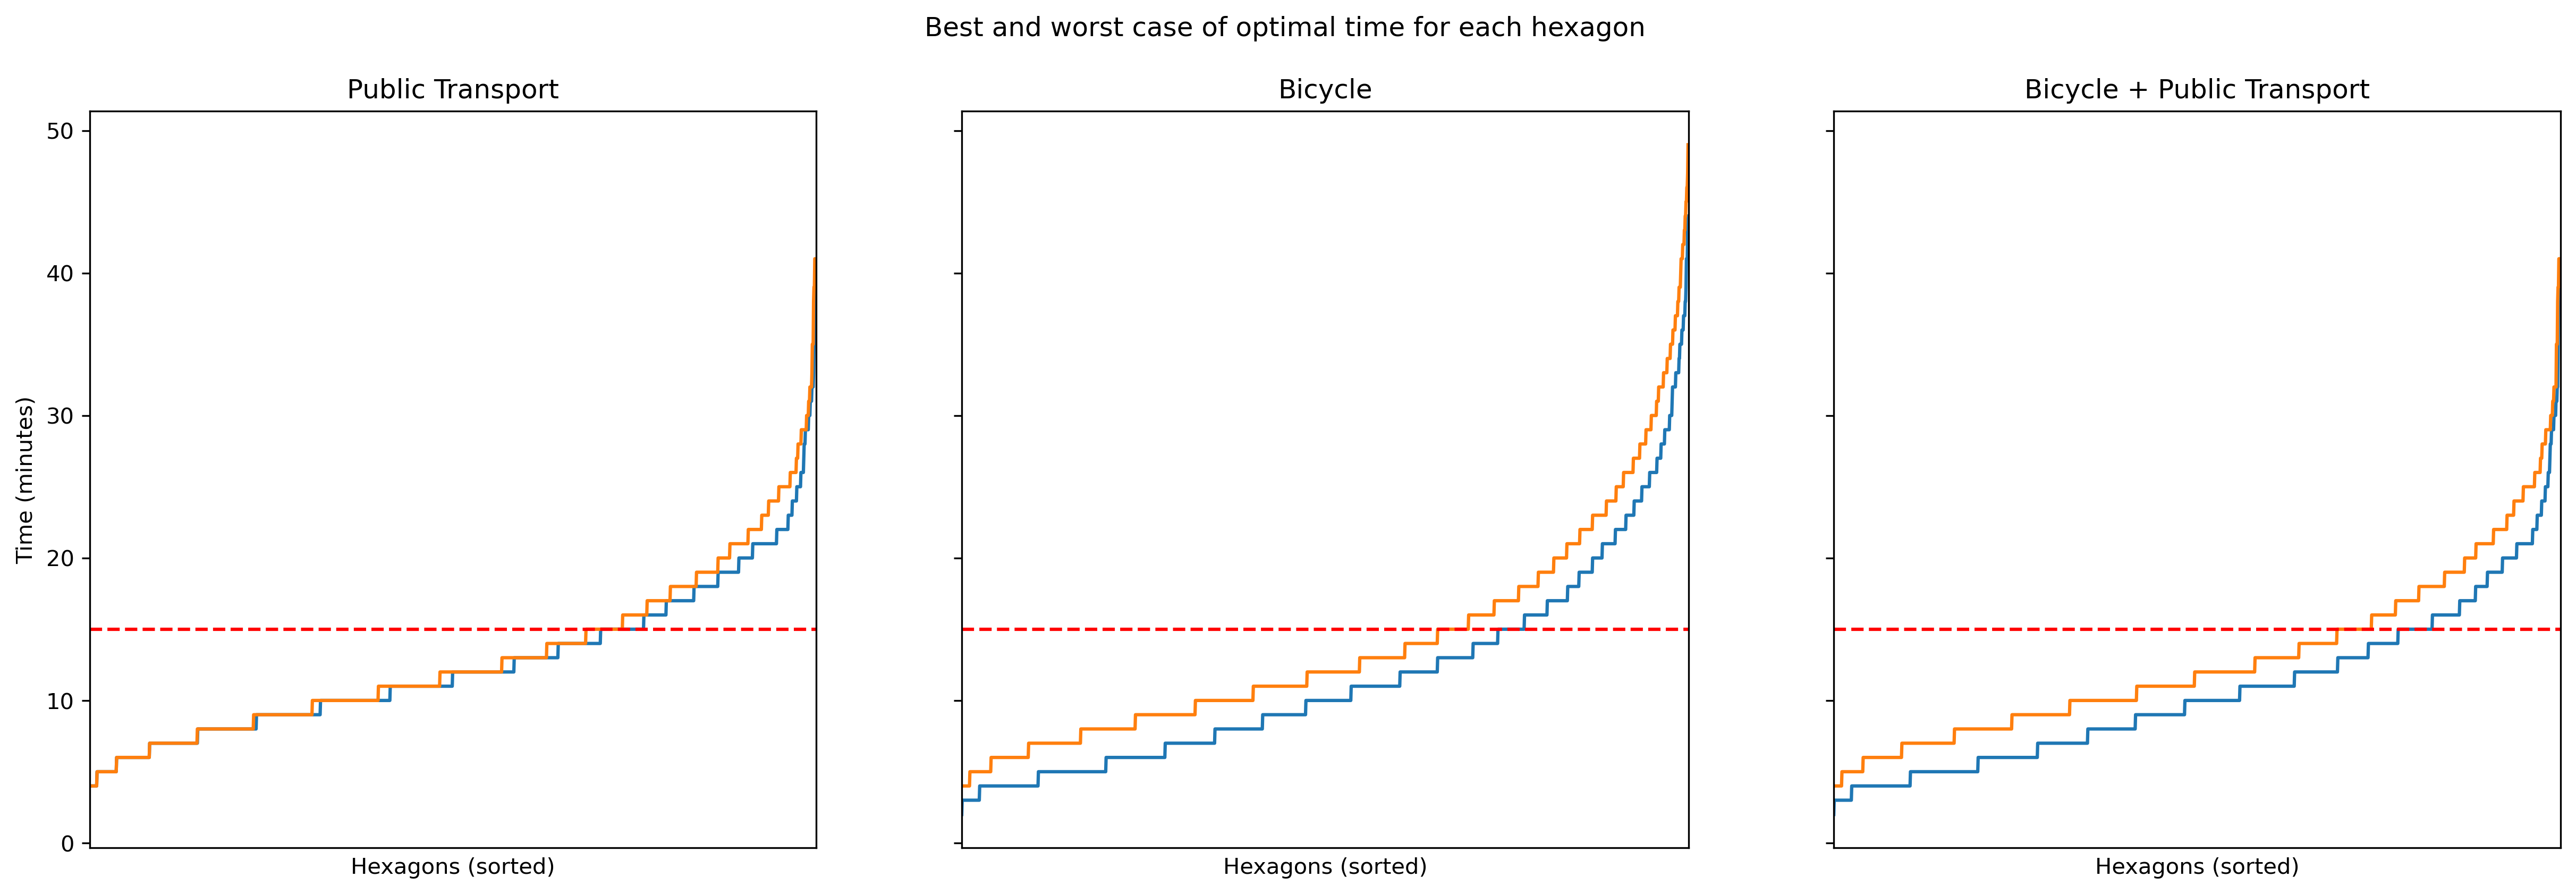
\includegraphics[width=0.95\textwidth]{Figures/results/uncertainty/optimal_best_worst_case}
  \end{center}
  \caption{Best and worst case of optimal time for each hexagon}
  \label{fig:best_and_worst_case_of_optimal_time_for_each_hexagon}
\end{figure}

First, we see that the variation for bicycles is spread out over almost all hexagons, in comparison to public transport where the variation only really begins to happen after the 15-minute mark.
For the combined scenario, we see the expected: the variances of the public transport scenario and the bicycle scenario add up.
